\documentclass[letterpaper]{article}
\usepackage{amsmath, amsthm}
\usepackage{mathtools}
\usepackage{tikz}

\DeclareGraphicsExtensions{.png}

\newtheorem{thm}{Theorem}
\newtheorem{lem}[thm]{Lemma}

\begin{document}

\begin{center}
\large\bf University of Waterloo\\
CS~798 --- Mathematical Foundations of Computer Networking\\
Winter 2014\\
Assignment 1\\
Siwei Yang - 20258568\\
\end{center}
\bigskip

\begin{enumerate}
\item{Problem 1}

\begin{enumerate}
\item{} The activities in a system are observed for a time period of length L (from 0 to L).
Let:
\begin{itemize}
\item n = number of jobs arrived in (0, L) = number of jobs processed in (0, L) 
\item $a_j$ = probability that an arriving job sees j jobs in the system
\item $d_j$ = probability that a departing job leaves behind j jobs in the system
\end{itemize}
There are no group arrivals (i.e., jobs arrive one after another). Show that $a_j$ = $d_j$ for all j.

Let $h_i$ be the number of jobs in the system when the $i^{th}$ job arrives, and $b_i$ be the number of jobs in the system when the $i^{th}$ job leaves the system. Of course, realistically, the order job arrives and departures have nothing to do with each other. However

\begin{lem}
we can alter the order job leaves the system without affecting $a_j, d_j$
for any scenario
\end{lem}

So, re-order the job departures so that it is always the last arriving job that leaves the system first. This gurantees every job sees the same number of jobs when both arriving and leaving the system. In other words, for any job, jobs arriving after it will leave system before it too. And jobs it sees on arrival will not leave system until it leaves. Therefore we have

\begin{equation}
\forall i . h_i = b_i
\end{equation}

Also we know that

\begin{equation}
a_i = \mid \{h_j \mid h_j = i\} \mid
\end{equation}

\begin{equation}
d_i = \mid \{b_j \mid b_j = i\} \mid
\end{equation}

Thus, given $h_i = b_i$, we can conclude that $a_i = d_i$ for all $i$.
\item{} Suppose arrivals occur in groups of two (i.e., we always see two jobs arriving at the same time), and we assume that both arriving jobs see the same number of jobs in the system. Is the relationship $a_j$ = $d_j$ for all j still true for this case? Explain your answer.

The relationship is not true any more. A simple counter example can be given for the case that only 2 jobs in total. So we have:
\begin{equation}
h_0=h_1=0 \text{ and }b_0=1,b_1=0
\end{equation}
Therefore, we calculate $a_0=1$ and $d_0=\frac{1}{2}, d_1=\frac{1}{2}$ which are not equal.

\end{enumerate}
\medskip

\item{Problem 2}

Suppose there are n arrivals in a time period of length L (from 0 to L), and the $n^{th}$ arrival (or last arrival) occurs at time L. Let $t_1$ be the time between 0 and the time of the first arrival, and $t_i$ be the interarrival time between the $(i-1)^{st}$ and $i^{th}$ arrivals, $i = 2, 3, \dotsc, n$
\begin{enumerate}
\item{} Let X be the time until the next arrival. Plot X as a function of time t for $0 \le t \le L$.

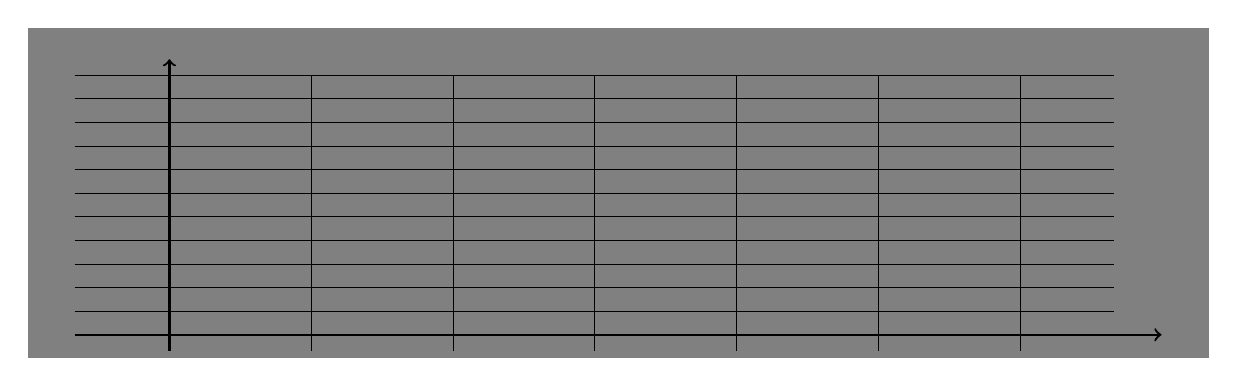
\begin{tikzpicture}[domain=0:1,yscale=1,xscale=6,smooth]
\fill[gray] (-1.2,-1.2) rectangle (1.3,3);
\draw[very thin] (-1.1,-1.1) grid[step=.3] (1.1,2.4);
\draw[thick,->] (-1.1,-0.9) -- (1.2,-0.9);
\draw[thick,->] (-0.9,-1.1) -- (-0.9,2.6);
\draw[color=red] plot[id=1] function{cos(pi*x)};
\end{tikzpicture}

\item{} Let $E[Y] = \frac{1}{n} * \sum^{n}_{i=1}{t_i}$ and $E[Y^2] = \frac{1}{n} * \sum^{n}_{i=1}{t_i^2}$ be the mean and second moment of the interarrival time, respectively. Using the plot in part (a), obtain an expression for E[X], the mean of X, as a function of E[Y] and E[Y2].
\begin{equation}
E[X] * L = \int_{0}^{L}{X}
\end{equation}

In other words, $E[X] * L$ equals to the bounded regions in plot of part a.
\begin{equation}\label{eq:region}
E[X] * L = \sum_{1}^{n}{\frac{t^2}{2}}
\end{equation}

and we know that
\begin{equation}\label{eq:region-sum}
E[Y] * n = L, E[Y^2] * n = \sum^{n}_{i=1}{t_i^2}
\end{equation}

Combine equation \ref{eq:region} and equation \ref{eq:region-sum} together, we end up with
\begin{equation}
E[X] = \frac{E[Y^2]}{2 * E[Y]}
\end{equation}

\end{enumerate}
\medskip

\item{Problem 3}
\begin{enumerate}
\item{} Consider a single server queue model with two classes of jobs. Let $n_j$ = number of class j jobs arrived in $(0, L)$ = number of class j jobs processed in $(0, L)$, j = 1, 2. Also let $x_{ij}$ be the service time of the $i^{th}$ class j job. Obtain analytic results for $U_j^{'}$, the utilization of the server by class j jobs, j = 1, 2.

we have
\begin{equation}
U = \frac{1}{L} * \sum_{j=1}^{n}{x_j}
\end{equation}
for the general server utilization. But taking account the setting in problem statement, given the two classes of jobs, we alter the formula to get
\begin{equation}
U_j' = \frac{1}{L} * \sum_{i=1}^{n_j}{x_{ij}}
\end{equation}
\begin{minipage}{\textwidth}
\item{} Consider a queueing model with a single queue and two parallel servers (see Figure below). Let n = number of jobs arrived in (0, L) = number of jobs processed in (0, L). Also let $x_i$ be the service time of the $i^{th}$ job. Is it possible to obtain analytic results for $U_i$, the utilization of server i, i = 1, 2? Explain your answer.
\includegraphics[width=\textwidth]{a1q3.png}
\end{minipage}

Assuming the single queue is FIFO, and it dispatches job to idle server(always server 1 when both are idle), we can only determine the job scheduling if the arrival time of each job is known. But without the arrival time, the utilization of server 1 and 2 can be totally different while the service time of each job remains constant.

Consider:

\begin{tabular}{l*{6}{c}r}
Job              & service time & arrival time \\
\hline
job 1            & 3 & 0 \\
job 2            & 3 & 3 \\
\end{tabular}

\begin{tabular}{l*{6}{c}r}
Job              & service time & arrival time \\
\hline
job 1            & 3 & 0 \\
job 2            & 3 & 0 \\
\end{tabular}

in the first scenario, server 1 have full utilization while in the second case server 1 and 2 splt utilization evenly.

\end{enumerate}
\medskip

\begin{minipage}{\textwidth}
\item{Problem 4}

Consider the tandem queue model shown in the Figure below. Packets sent by the sender are transmitted along a path consisting of links 1, 2, 3 and 4, and then delivered to the receiver. Each link is modeled by a server.

\includegraphics{a1q4.png}
\end{minipage}
Suppose link 3 is under heavy load and the loss probability at link 3 is p (the loss probabilities at the
other three links are zero). Let
\begin{itemize}
\item{} Y be the system throughput = the rate at which packets are delivered to the receiver
\item{} R be the mean end-to-end delay from sender to receiver
\item{} Q be the mean number of packets in the network
\end{itemize}
It has been suggested that according to Little'’s Law, we can write $YR = Q$. Do you agree? Explain your answer.

I do not agree.

Little'’s Law is building on the idea that we can represent the total amount of time that every job spend in the system in two ways. However, for $Y, R$ define in this problem, only the sucessful jobs are accounted for. While $Q$ receives contribution from dropped packets too. Therefore, two sides of the equation does not agree on the total amount of time that they are using. Put that into equations we can have:
\begin{equation}
YR = \lambda * (1 - p) * R
\end{equation}
\begin{equation}
Q = \lambda * (1 - p) * R + \lambda * p * R'
\end{equation}
where $\lambda$ is the total arrival rate to the system, and $R'$ is the mean response time for dropped packets. Thus, we can conclude from the equations that $YR = Q$ does not hold unless $p = 0$.
\medskip

\begin{minipage}{\textwidth}
\item{Problem 5}
Consider the following open queueing network model. Suppose the mean response times at the four servers, denoted by $R_1$, $R_2$, $R_3$, and $R_4$, are 0.02, 0.03, 0.05, and 0.02 seconds, respectively. For this model, the end-to-end delay is the elapsed time from when a job arrives from outside the network to when this job departs from the network. Determine R, the mean end-to-end delay.

\includegraphics[width=\textwidth]{a1q5.png}
\end{minipage}

Let $\lambda$, $\lambda_1$, $\lambda_2$, $\lambda_3$, $\lambda_4$ to be total arrival rate for whole system and server 1, 2, 3, 4 respectively. Then we have equations:

\begin{equation}
\lambda_1 = 1 + \lambda_2 + \lambda_3 + \lambda_4
\end{equation}

\begin{equation}
\lambda_2 = \lambda_1 * p_{12}
\end{equation}

\begin{equation}
\lambda_3 = \lambda_1 * p_{12}
\end{equation}

\begin{equation}
\lambda_4 = \lambda_1 * p_{12}
\end{equation}

By solving this system of euqations, we have $\lambda_1 = 20$, $\lambda_2 = 8$, $\lambda_3 = 7$, $\lambda_4 = 4$. Also from the problem statement we have:
\begin{equation}
\gamma = \gamma_1 = 1
\end{equation}
Combine with the response time formula derived from Little''s Law:
\begin{equation}
R = \frac{1}{\gamma} * \sum_{i=1}^{M}{\lambda_i * R_i}
\end{equation}
we have the total response time being $20 * 0.02 + 8 * 0.03 + 7 * 0.05 + 4 * 0.02 = 1.07$.
\medskip

\item{Problem 6}

\begin{enumerate}
\item{} Consider a queueing model with a single server, two classes of jobs, and cyclic service discipline. This is illustrated in the diagram below.

\includegraphics{a1q6.png}
Under cyclic service, class 1 job arrivals join queue 1 and class 2 job arrivals join queue 2. Service is provided in cycles. A cycle starts with the server checking queue 1. If queue 1 is non-empty, the first job at queue 1 is processed. The server then checks queue 2 and processes the first job at queue 2 if queue 2 is non-empty. The cycle ends when processing of this job is complete.

The cycle time is defined to be the sum of:
\begin{itemize}
\item{} Service time of first job at queue 1 (if queue 1 is non-empty), and zero otherwise
\item{} Service time of first job at queue 2 (if queue 2 is non-empty), and zero otherwise
\item{} Time spent in moving from queue 1 to queue 2 and back to queue 1
\end{itemize}

Suppose there are K cycles in a time period of length L (from 0 to L). Let
\begin{itemize}
\item{} m = number of class 1 jobs arrived in (0, L) = number of class 1 jobs processed in (0, L)
\item{} n = number of class 2 jobs arrived in (0, L) = number of class 2 jobs processed in (0, L)
\item{} $s_i$ = service time of the $i^{th}$ class 1 job, $i = 1, 2, \dotsc, m$
\item{} $x_j$ = service time of the $j^{th}$ class 2 job, $j = 1, 2, \dotsc, n$
\item{} H = time spent in moving from queue 1 to queue 2 and back to queue 1; H is a constant regardless of whether queue 1 is empty or not, or whether queue 2 is empty or not.
\end{itemize}

Also let
\begin{itemize}
\item{} $S_1^{'}$ = mean service time of class 1 jobs
\item{} $S_2^{'}$ = mean service time of class 2 jobs
\item{} C = mean cycle time
\item{} $\lambda_1^{'}$ = arrival rate of class 1 jobs
\item{} $\lambda_2^{'}$ = arrival rate of class 2 jobs
\end{itemize}
Derive an analytic expression for C. You must express your answer as a function of H, $S_1^{'}$, $S_2^{'}$, $\lambda_1^{'}$ and $\lambda_2^{'}$ only.

Consider the total running time of the server:
\begin{equation}
T = K * H + S_1^{'} * m + S_2^{'} * n = C * K
\end{equation}

Also, we know that:
\begin{equation}
m = C * K * \lambda_1^{'}
\end{equation}
\begin{equation}
n = C * K * \lambda_2^{'}
\end{equation}

Combining all three equations gives:
\begin{equation}
H + S_1^{'} * C * \lambda_1^{'} + S_2^{'} * C * \lambda_2^{'} = C
\end{equation}

Therefore, the mean cycle time is $\frac{H}{1 - S_1^{'} * \lambda_1^{'} - S_2^{'} * \lambda_2^{'}}$.

\item{} Repeat part (a) for the case of a cyclic service discipline with exhaustive service. Under exhaustive
service, each time queue j is checked during a cycle ($j = 1, 2$), jobs at queue j are processed until queue
j is empty. For this case, the cycle time is the sum of:
\begin{itemize}
\item{} Total service time of jobs at queue 1 that have been processed (if queue 1 is non-empty), and zero otherwise
\item{} Total service time of jobs at queue 2 that have been processed (if queue 2 is non-empty), and zero otherwise
\item{} Time spent in moving from queue 1 to queue 2 and back to queue 1
\end{itemize}
Derive an analytic expression for C. You must express your answer as a function of H, $S_1^{'}$, $S_2^{'}$, $\lambda_1^{'}$ and $\lambda_2^{'}$ only.

All three equations in part(a) still hold, so the expression for C will not change. It remains $\frac{H}{1 - S_1^{'} * \lambda_1^{'} - S_2^{'} * \lambda_2^{'}}$.
\end{enumerate}
\medskip

\item{Problem 7}

Consider the following closed queueing network with N circulating jobs.

\includegraphics{a1q7.png}
Let $S_i$ be the mean service time at server i, i = 1, 2, and 3. Consider the case where $S_1$ = 0.3 second, $S_2$ = 0.6 second, and $S_3$ = 0.4 second.
\begin{enumerate}
\item{} When N = 1, what are the values of $\lambda_i$, $R_i$, and $Q_i$, the arrival rate to server i, the mean response time at server i, and the mean number of jobs at server i, respectively, for i = 1, 2, and 3?

When $N = 1$, there's no waiting time for jobs to be processed. In other words, service time is the same as response time. So we have:
\begin{equation}
R_1 = S_1 = 0.3
\end{equation}
\begin{equation}
R_2 = S_2 = 0.6
\end{equation}
\begin{equation}
R_3 = S_3 = 0.4
\end{equation}
Then, mean service cycle takes time in seconds $C = R_1 + R_2 + R_3 = 1.3$. This give us the through put/arrival rate of the system:
\begin{equation}
\frac{1}{C} = Y = \lambda = \frac{10}{13}
\end{equation}
Since this is a simple circular network, we have $\lambda = \lambda_1 = \lambda_2 = \lambda_3 = \frac{10}{13}$. Then apply Little's Law, we get $Q_1 = \lambda_1 * S_1 = \frac{3}{13}$, $Q_2 = \lambda_2 * S_2 = \frac{6}{13}$, $Q_3 = \lambda_3 * S_3 = \frac{4}{13}$.

\item{} Give the upper bound utilization for each of the three servers.
We know that utilization of any server is at most 1. And
\begin{equation}
\frac{U_1}{U_2} = \frac{S_1}{S_2} = 0.5
\end{equation}
\begin{equation}
\frac{U_3}{U_2} = \frac{S_3}{S_2} = \frac{2}{3}
\end{equation}
Therefore, the upper bound utilization for the 3 servers are: $U_1 = 0.5$, $U_2 = 1$, $U_3 = \frac{2}{3}$.

\end{enumerate}
\medskip

\item{Problem 8}

Consider the web application model described in the lecture notes entitled "“Queueing Models -– Analytic Results"”. The transition probabilities are $p_{10} = 0.2$, $p_{12} = 0.8$, $p_{01} = p_{21} = 1$; all others have value zero. The mean think time is 5 seconds, and the mean service times per visit to the web/application server and the database server are 0.05 and 0.1 seconds, respectively.

First solve for the relative traffice on each of the servers. Let $\lambda_0$, $\lambda_1$ and $\lambda_2$ be the job arrival rate for server 0, 1, 2 respectively. Then we have:
\begin{equation}
\lambda_1 = p_{01} * \lambda_0 + p_{02} * \lambda_2
\end{equation}
\begin{equation}
\lambda_0 =  p_{10} * \lambda_1
\end{equation}
\begin{equation}
\lambda_2 = p_{12} * \lambda_1
\end{equation}
And the total yield or arrival rate to the system is the same as the rate jobs enter thinking state:
\begin{equation}
\lambda = \lambda_0
\end{equation}
Therefore we have $\lambda_2 = 4 * \lambda_0$ and $\lambda_1 = 5 * \lambda_0$. And we know the total yield $Y = \lambda = \lambda_0$. Referring to Little's Law for multiple servers:
\begin{equation}
R = \frac{\lambda_1 * R_1 + \lambda_2 * R_2}{Y} = \frac{\lambda_1}{\lambda_0} * R_1 + \frac{\lambda_2}{\lambda_0} * R_2 = 5 * R_1 + 4 * R_2
\end{equation}
where $R_1$ and $R_2$ are mean response time for server 1, 2 respectively. Also consider the server utilization:
\begin{equation}
U_i = \lambda_i * S_i
\end{equation}
and we can solve for the relative utilization of $\frac{U_1}{U_2} = \frac{5 * S_1}{4 * S_2}$. Lastly, we know that finite population model obeys the following equation:
\begin{equation}\label{eq:pop-time}
\lambda * (R + Z) = N
\end{equation}

\begin{enumerate}
\item{} Derive a lower bound for the mean response time R as a function of N, the number of user workstations.

$R_1$ and $R_2$ are bounded by the mean service time of server 1, 2, and is achievable when there is only one job. And, R is lower bounded by $R_1$ and $R_2$. Thus, we have the lower bound of R when $R_1 = 0.05$ and $R_2 = 0.1$ which gives us $R = 0.25 + 0.4 = 0.65$.

Let's consider system saturation point $N^*$. We have relative utilization of $\frac{U_1}{U_2} = \frac{5}{8}$. Therefore, $N^*$ is reached when $U_2 = 1$ and we have equation for it:
\begin{equation}
\lambda_2 * S_2 = 1
\end{equation}
And we substitue the solved value of $\lambda = 2.5$ and the minimum response time of $R = 0.65$ into equation \ref{eq:pop-time} to get  $N^* = 14.125$.

Beyound the saturation point, the yield of system would stay the same while the response time increases linearly with respect to population. We have equation \ref{eq:pop-time} describing the relationship given a maximized yield at $\lambda = 2.5$. Therefore, we have the lower bound for R as:
\begin{equation*}
R = \begin{cases}
               0.65                                      & n \le 14.125\\
               \frac{N}{2.5} - 5                    & n \ge 14.125
           \end{cases}
\end{equation*}

\item{} Suppose the web/application server is deployed on a machine that is twice as fast (i.e., the mean service time at the web/application server is 0.025 second instead of 0.05 second). The values of the other parameters remain unchanged. Derive a lower bound for the mean response time R as a function of N.

$R_1$ and $R_2$ are bounded by the mean service time of server 1, 2, and is achievable when there is only one job. And, R is lower bounded by $R_1$ and $R_2$. Thus, we have the lower bound of R when $R_1 = 0.025$ and $R_2 = 0.05$ which gives us $R = 0.325$.

Let's consider system saturation point $N^*$. We have relative utilization of $\frac{U_1}{U_2} = \frac{5}{8}$. Therefore, $N^*$ is reached when $U_2 = 1$ and we have equation for it:
\begin{equation}
\lambda_2 * S_2 = 1
\end{equation}
And we substitue the solved value of $\lambda = 5$ and the minimum response time of $R = 0.325$ into equation \ref{eq:pop-time} to get  $N^* = 26.625$.

Beyound the saturation point, the yield of system would stay the same while the response time increases linearly with respect to population. We have equation \ref{eq:pop-time} describing the relationship given a maximized yield at $\lambda = 5$. Therefore, we have the lower bound for R as:
\begin{equation*}
R = \begin{cases}
               0.325                                   & n \le 26.625\\
               \frac{N}{5} - 5                      & n \ge 26.625
           \end{cases}
\end{equation*}

\item{} Suppose the database server is deployed on a machine that is twice as fast (i.e., the mean service time at the database server is 0.05 second instead of 0.1 second). The values of the other parameters remain unchanged. Derive a lower bound for the mean response time R as a function of N.

$R_1$ and $R_2$ are bounded by the mean service time of server 1, 2, and is achievable when there is only one job. And, R is lower bounded by $R_1$ and $R_2$. Thus, we have the lower bound of R when $R_1 = 0.05$ and $R_2 = 0.05$ which gives us $R = 0.45$.

Let's consider system saturation point $N^*$. We have relative utilization of $\frac{U_1}{U_2} = \frac{5}{4}$. Therefore, $N^*$ is reached when $U_1 = 1$ and we have equation for it:
\begin{equation}
\lambda_1 * S_1 = 1
\end{equation}
And we substitue the solved value of $\lambda = 4$ and the minimum response time of $R = 0.45$ into equation \ref{eq:pop-time} to get  $N^* = 21.8$.

Beyound the saturation point, the yield of system would stay the same while the response time increases linearly with respect to population. We have equation \ref{eq:pop-time} describing the relationship given a maximized yield at $\lambda = 4$. Therefore, we have the lower bound for R as:
\begin{equation*}
R = \begin{cases}
               0.45                                     & n \le 21.8\\
               \frac{N}{4} - 5                      & n \ge 21.8
           \end{cases}
\end{equation*}

\item{} Explain the similarity (or difference) of the three lower bounds obtained in parts (a), (b), and (c).

parts (a), (b) both have full saturation when server 2 is at 100\% utilization even though the server capacities are doubled in part(b). In part (c), the change of relative speed between server 1 and 2 moved the full saturation to 100\% utilization of server 1. Once we figured out the full saturation point for each part, the rest is plug numbers into equation \ref{eq:pop-time} to obtain the rate of growth of response time.
\end{enumerate}

\end{enumerate}
\end{document}

